\documentclass[german,a4paper]{llncs}

\usepackage{german}
\usepackage{palatino}
\usepackage[T1]{fontenc}
\usepackage[utf8x]{inputenc}
\usepackage{graphicx, wrapfig} 							% Grafikpaket und Grafik im Textfluß
\usepackage{bibgerm}
\usepackage[footnote, nolist]{acronym}                   % Abkürzungen
\usepackage{tabularx,longtable, multirow} 				% Tabellen
\renewcommand\arraystretch{1.4}                          % Tabellen Zeilenhöhe
\newcolumntype{C}[1]{>{\hsize=#1\hsize\centering\arraybackslash}X} % Spalte zentrieren
\newcolumntype{L}[1]{>{\hsize=#1\hsize\raggedright\arraybackslash}X}%
% Seitenränder
\usepackage{geometry}
\geometry{verbose,a4paper,tmargin=5.2cm,bmargin=5.2cm,lmargin=4.4cm,rmargin=4.4cm}

% Kopf- und Fusszeile
\usepackage{fancyhdr}
\pagestyle{fancy}
\renewcommand{\headrulewidth}{0pt}
\renewcommand{\footrulewidth}{0pt}
\fancyhead[EL]{\textsc{Fabian Schneider}}				% Hier bitte den/die Autor(en) angeben
\fancyhead[OR]{\textsc{CDR}}								% Hier bitte den Dokumententitel angeben
\fancyfoot[EC,OC]{}

\usepackage{listingsutf8, color}
\renewcommand*\lstlistingname{Beispielcode}
\definecolor{mygray}{rgb}{0.9,0.9,0.9}
\lstset{language=Java,
		backgroundcolor=\color{mygray},   % choose the background color; you must add \usepackage{color} or \usepackage{xcolor}
        basicstyle=\footnotesize,         % the size of the fonts that are used for the code
        breaklines=true,
        tabsize=4,
        numbers=left,
        stepnumber=2,
}
\lstset{prebreak=\raisebox{0ex}[0ex][0ex]
        {\ensuremath{\hookleftarrow}}}
\lstset{postbreak=\raisebox{0ex}[0ex][0ex]
        {\ensuremath{\hookrightarrow\space}}}


\usepackage{hyperref}	
											% Links ins Internetz
\begin{document}

% Titel
\title{CDR}															% Hier bitte den Dokumententitel angeben
\subtitle{Contexts and Dependency Remoting}							% Hier bitte den Untertitel angeben
\author{Fabian Schneider}					    						% Hier bitte den/die Autor(en) angeben; mehrere bitte durch Komma trennen
\institute{Universität Ulm, Institut für Datenbanken und Informationssysteme\\
           \email{Fabian-2.Schneider@uni-ulm.de}}					% Hier bitte die EMail-Adresse(n) des/der Autors/Autoren angeben
           
\maketitle

\begin{acronym}
	\acro{REST}{Representational State Transfer}
	\acro{CDI}{Contexts and Dependency Injection}
	\acro{CDR}{Contexts and Dependency Remoting}
	\acro{JAX-RS}{Java API for RESTful Web Services}
	\acro{JVM}{Java virtual machine}
	\acro{JSON}{JavaScript Object Notation}
	\acro{XML}{Extensible Markup Language}
	\acro{Java EE}{Java Platform, Enterprise Edition}
	\acro{HTTP}{Hypertext Transfer Protocol}
	\acro{URI}{Uniform resource identifier}
\end{acronym}

% Zusammenfassung
\begin{abstract}
Um in verteilten Softwaresystemen Komponente lose gekoppelt entwickeln zu können, ist es wichtig dass die Implementierungen frei von den Details der verschiedenen Bereitstellungsvarianten des Softwaresystems sind. 
\ac{CDR} ist ein Entwurfsmuster, das für diese Problemstellung durch de Kombination der Technologien \ac{CDI} und \ac{JAX-RS} einen Lösungsansatz bietet. 
\ac{JAX-RS} ermöglicht die Kommunikation mit entfernten Komponenten über eine \ac{REST}-Schnittstelle. 
Der \ac{CDI}"=Mechanismus stellt zur Laufzeit abhängig von der Bereitstellungsvariante eine Referenz auf eine lokale oder eine entfernte Komponente bereit.
\end{abstract}

% ab hier beginnt der eigentlich Text
\section{Einleitung}

\section{Konzept}
%\subsection{Technologien}
%\subsection{Aufbau}
\begin{figure}
\centering
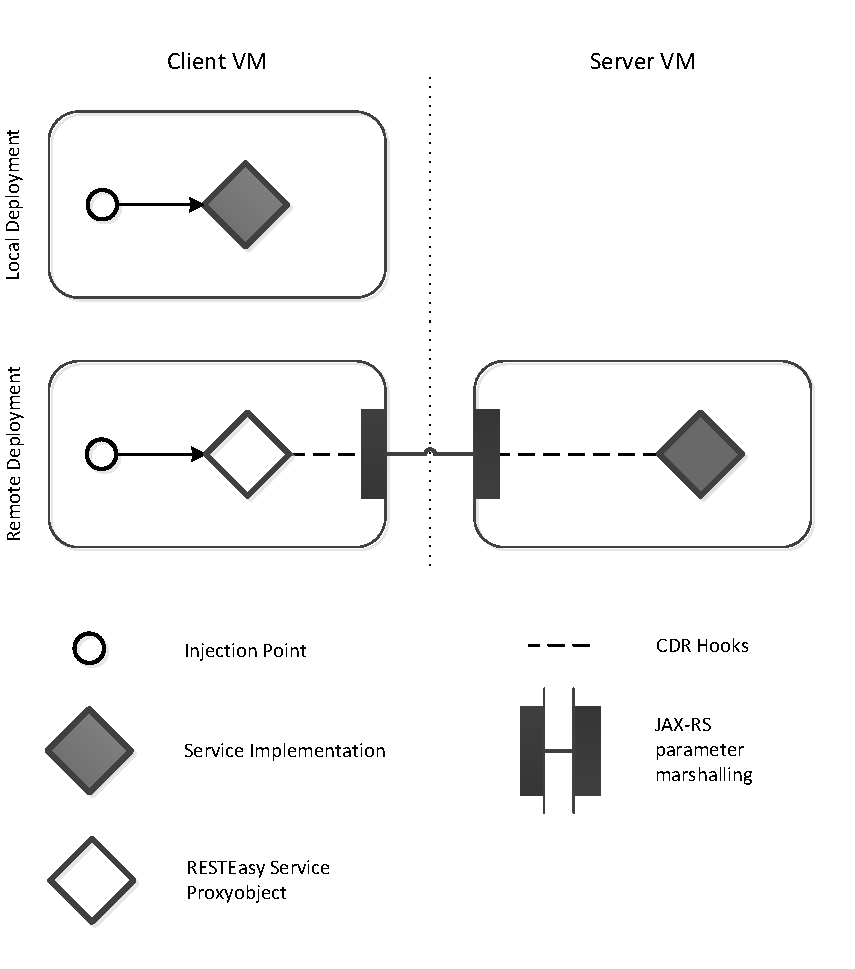
\includegraphics[width=0.8\textwidth]{img/CDR}
\caption{Architektur CDR\label{pic:cdr}}
\end{figure}
Abbildung \ref{pic:cdr} zeigt schematisch die Funktionsweise des \ac{CDR}"=Entwurfsmusters. Der Anwendungsfall wird durch den Beispielode \ref{lst:usecase} aufgezeigt und ist die Verwendung einer Komponente, die die Schnittstelle \textit{Service} implementiert.
\begin{lstlisting}[caption={Anwendungsfall CDR},captionpos=b,label=lst:usecase] 
@Inject
Service srv;
...
srv.doSomething();
\end{lstlisting}
Es werden die zwei Bereitstellungsvarianten \textit{Local deployment} und \textit{Remote deployment} unterschieden. 
Die Variante \textit{Local deployment} beschreibt ein Szenario, bei dem die Nutzung und die Breitstellung der \textit{Service}"=Komponente in der selben \ac{JVM} stattfinden. Ein \textit{Remote deployment} liegt demnach vor, wenn die \textit{Service}"=Komponente in einer von der Implementierung entfernten \ac{JVM} genutzt wird.\\ 
Die Variante \textit{Local deployment} ist der Standardfall. 
In der Client"=\ac{JVM} wird eine Implementierung der \textit{Service}"=Schnittstelle bereitgestellt, hier \textit{Service implementation}. 
Der \ac{CDI}"=Mechanismus kann die Abhängigkeiten ohne weitere Informationen auflösen. Es sind keine Anpassungen oder Annotationen am Quellcode notwendig.\\
Bei der Variante \textit{Remote deployment} wird im Beispielcode \ref{lst:usecase} eine Referenz auf ein Stellvertreterobjekt injiziert. 
Dieses Stellvertreterobjekt kommuniziert mit der Implementierung der \textit{Service}"=Komponente, die in der \textit{Server JVM} bereitgestellt wird. 
In beiden \ac{JVM}s bietet das \ac{CDR}-Entwurfsmuster die Möglichkeit eigenen Code auszuführen (\textit{CDR hook}), um die Parameter, Rückgabewerte oder Exceptions nach Bedarf zu transformieren. Dadurch können die in Kapitel \ref{sec:introduction} definierten Ziele wie transparente \textbf{Methodensignaturen} und \textbf{Exceptions} realisiert werden.
Die Kommunikation über die Grenzen der \ac{JVM}s hinweg wird durch die \ac{JAX-RS}"=Technologien realisiert, die auch eine transparente \textbf{Serialisierung} der übertragenen Objekte im \ac{JSON}"= oder \ac{XML}"=Format ermöglichen.
Für ein \textit{Remote deployment} werden in der \textit{Client JVM} die \textit{Service}"=Schnittstelle und die \ac{CDR}"=Komponenten bereitgestellt. 
In der \textit{Server JVM} wird die Implementierung der \textit{Service}"=Schnittstelle und die notwendigen \textit{CDR hooks} der Serverseite bereitgestellt.\\
Die Entscheidung über die Art der Bereitstellung hat keine Auswirkung auf die Anwendungslogik und kann daher für jeden Fall individuell getroffen und im Nachhinein auch wieder geändert werden.
Dadurch dass ein \textit{Local deployment} als Standardfall angenommen wird und alle Änderungen für ein \textit{Remote deployment} nicht die Anwendungslogik berühren, kann das \ac{CDR}"=Entwurfsmuster auch bei Bedarf leicht nachträglich ergänzt werden.
Die notwendigen Anpassungen werden in Kapitel \ref{sec:implementation} aufgezeigt.

\section{Umsetzung\label{sec:implementation}}
\begin{table}
\caption{\label{tab:project}Projektaufbau der Implementierung}
\begin{tabular}{lp{2cm}p{8cm}}
cdr-main &             & \\
|\_      & cdr-lib     & \ac{CDR}"=Komponenten.\\
|\_      & service-api & \textit{Service}"=Schnittstelle.\\
|\_      & service-lib & Implementierung der \textit{Service}"=Schnittstelle.\\
|\_      & cdr-poc     & Beinhaltet die Testfälle zur Veranschaulichung des \ac{CDR}"=Entwurfsmusters und die für \textit{Service} spezifische \textit{CDR hooks}.\\
\end{tabular}
\end{table}
Eine Beispielimplementierung des \ac{CDR}"=Entwurfsmusters in Java ist unter \href{https://github.com/Robotregent/cdr}{https://github.com/Robotregent/cdr} zu finden. 
Tabelle \ref{tab:project} zeigt den Aufbau des Mavenprojekts und den Zweck der einzelnen Module.
Die Funktionsweise der Beispielimplementierung wird an Hand zweier Testfälle aufgezeigt. Der erste Testfall zeigt wie eine lokale Bereitstellung für die Beispielkomponenten aufgebaut ist, der zweite Testfall zeigt die entfernte Bereitstellung nach dem \ac{CDR}"=Entwurfsmusters.
Um die Testfälle ausführen zu können, muss ein JBoss Anwendungsserver in der Version 7.1.1\footnote{\href{http://download.jboss.org/jbossas/7.1/jboss-as-7.1.1.Final/jboss-as-7.1.1.Final.zip}{{http://download.jboss.org/jbossas/7.1/jboss-as-7.1.1.Final/jboss-as-7.1.1.Final.zip}}} verfügbar sein.  
Der Befehl \colorbox{mygray}{\lstinline!mvn install!}, ausgeführt im Ordner \textit{cdr-main}, installiert alle restlichen Abhängigkeiten, übersetzt das Projekt und führt die Testfälle aus.\\
Im Folgenden werden die notwendigen Anpassungen für eine Umsetzung des \ac{CDR}"=Entwurfsmusters aufgezeigt.
\paragraph{Aktivierung}
Um eine Schnittstelle für das \ac{CDR}"=Entwurfsmuster zu aktivieren, muss diese mit \ac{JAX-RS} Annotationen erweitert werden. 
Beispielcode \ref{lst:activation} zeigt dies für die \textit{Service}"=Komponente.
\begin{lstlisting}[caption={Aktivierung},captionpos=b,label=lst:activation] 
@Path("/")
public interface Service {	
	@GET
	@Path("/item")
	@Produces(MediaType.APPLICATION_JSON)
	public TodoItem[] getItems();	

	@POST
	@Path("/item")
	@Consumes(MediaType.APPLICATION_JSON)
	public Integer takeItem(TodoItem tdi);	
}
\end{lstlisting}
Die Methoden der Komponente werden mit Hilfe der Annotationen \colorbox{mygray}{\lstinline!@GET!} und \colorbox{mygray}{\lstinline!@POST!} den entsprechenden \ac{HTTP}"=Methoden zugeordnet. \colorbox{mygray}{\lstinline!@Path!} bestimmt unter welcher \ac{URI} die annotierten Elemente zu erreichen sind. Weiterführende Informationen über die Gestaltung von \ac{REST}"=Schnittstellen und die Implementierung dieser mit \ac{JAX-RS} liefern Tilkov \cite{Tilkov2011} und Burke \cite{Burke2010}. \\
Die Annotationen \colorbox{mygray}{\lstinline!@Consumes!} und \colorbox{mygray}{\lstinline!@Produces!} steuern die Serialisierung der Parameter und werden im entsprechenden Abschnitt noch näher behandelt.
\newpage
\paragraph{Stellvertreterobjekt}
Der Beispielcode \ref{lst:factory} zeigt mit einem Ausschnitt der abstrakte Klasse \colorbox{mygray}{\lstinline!CDRFactory <T>!} die zentrale Komponente im \ac{CDR}"=Entwurfsmuster.
Die Methode \colorbox{mygray}{\lstinline!T produces()!} muss für jede Ausprägung der abstrakten Klasse implementiert werden und agiert als \textit{Producer}"=Methode des \ac{CDI}"=Mechanismus. Bei der Implementierung genügt es, die Methode \colorbox{mygray}{\lstinline!T getService (Class<T> clazz)!} aufzurufen, um das Stellvertreterobjekt zu erzeugen. 
Die \ac{CDI}"=Spezifikation legt in §3.3 fest, dass eine \textit{Producer}"=Methode keine Typvariable als Rückgabewert haben darf. Daher ist diese Indirektion notwendig. Siehe dazu auch \cite{group2009jsr299}.\\
In der Beispielimplementierung wird die \ac{URI} der entfernten Komponente über eine \textit{Properties}"=Datei aufgelöst. Hier sind auch andere Mechanismen wie z.B. Annotationen denkbar.\\ 
Die Methoden \colorbox{mygray}{\lstinline!registerClientInterceptor()!} und \colorbox{mygray}{\lstinline!registerClientExceptionMapper()!} sind die \textit{CDR hooks} Für den Client. 
\begin{lstlisting}[caption={Abstrakte CDR"=Fabrik},captionpos=b,label=lst:factory] 
public abstract class CDRFactory <T> {	

	protected abstract T produces();

	protected T getService (Class<T> clazz){							
				
		URI uri = getUri(clazz.getCanonicalName());			
		ClientRequestFactory crf = new ClientRequestFactory(UriBuilder.fromUri(uri).build());	
		
		registerClientInterceptor(crf);	
		
		ResteasyProviderFactory pf = ResteasyProviderFactory.getInstance();
		
		registerClientExceptionMapper(pf);		

		return crf.createProxy(clazz);
	}
	
	protected void registerClientInterceptor(ClientRequestFactory crf){
	}
	
	protected void registerClientExceptionMapper(ResteasyProviderFactory pf){
	}
}
\end{lstlisting}
\newpage
\paragraph{Methodensignaturen}
Die Konfiguration der \ac{HTTP}"=Kommunikation erfolgt bei \ac{JAX-RS} durch Annotation der Komponenten. Dies ermöglicht es, die Geschäftslogik frei von den Details der Bereitstellung zu halten.
Allerdings muss hier eine Abwägung zwischen Transparenz der Methodensignaturen und Aussagekraft der \ac{REST}"=Schnittstelle getroffen werden.
Die Beispielimplementierung nutzt die Möglichkeiten von \ac{JAX-RS} und \textit{resteasy}, um \ac{HTTP}"=Anfragen und "=Antworten unabhängig von der Geschäftslogik manipulieren zu können. Im Konzept werden diese Komponenten als \textit{CDR hooks} bezeichnet. 
Durch diesen Mechanismus können beide Ziele erreicht werden.\\
Das Manipulieren der \ac{HTTP}"=Anfrage ist über die in Beispielcode \ref{lst:factory} gezeigte Methode \colorbox{mygray}{\lstinline!registerClientInterceptor()!} möglich. Hier kann ein \textit{resteasy ClientExecutionInterceptor} registriert werden. Siehe dazu auch \cite{resteasy}.\\
Beispielcode \ref{lst:serverinterceptor} zeigt, wie die \ac{HTTP}"=Antwort durch einen \textit{CDR hook} auf der Serverseite manipuliert wird. Um die Aussagekraft der \ac{REST}"=Schnittstelle zu vergrößern, wird nach dem Erzeugen einer Ressource der entsprechende \ac{HTTP}"=Statuscode und \textit{Location"=Header} gesetzt. 
\begin{lstlisting}[caption={ServerPostProcessInterceptor},captionpos=b,label=lst:serverinterceptor] 
@Provider
@ServerInterceptor
public class ServerPostProcessInterceptor implements PostProcessInterceptor, AcceptedByMethod {	
	
	@Context
	HttpServletRequest request;
	
	public void postProcess(ServerResponse response) {
		Integer id = (Integer) response.getEntity();
		response.setStatus(201);
		MultivaluedMap<String, Object> headers = response.getMetadata();
		 
		String url = request.getRequestURL().toString();
		
		headers.add("Location", url );
	}
}
\end{lstlisting}

\paragraph{Exceptions}
Damit die Fehlerbehandlung transparent zur Bereitstellung bleibt, müssen die entsprechenden \textit{CDR hooks} implementiert werden. Ohne diese zusätzlichen Komponenten erzeugt die \ac{JAX-RS}"=Laufzeitumgebung nur eine generische Fehlernachricht. 
Der \ac{HTTP}"=Statuscode wäre 500 und auf der Seite des Clients würde der \textit{resteasy}"=Fehlertyp \textit{ClientResponseFailure} erzeugt werden. 
Dadurch würde die Semantik der Fehlerbehandlung in der Anwendung verloren gehen und die Geschäftslogik wäre nicht mehr frei von den Details der Bereitstellung. Diese Problematik kann durch die folgenden \textit{CDR hooks} umgangen werden:
\begin{description}
\item [ServerExceptionMapper] Wird von der \ac{JAX-RS}"=Laufzeitumgebung aufgerufen, wenn der entsprechende Fehler auftritt. Der Fehlertyp kann durch einen individuellen Statuscode in der \ac{HTTP}"=Antwort repräsentiert werden.
\item [ClientExceptionMapper] In der \ac{JVM} des Clients kann der Statuscode ausgelesen und der entsprechende Fehlertyp erzeugt werden. Allerdings ist dies nur für Fehlertypen möglich, die den Typ \textit{RuntimeExpetion} erweitern. Beispielcode \ref{lst:ClientExceptionMapper} zeigt einen Ausschnitt aus der Implementierung.
\end{description}
\begin{lstlisting}[caption={ClientExceptionMapper},captionpos=b,label=lst:ClientExceptionMapper] 
public class ClientExceptionMapper implements ClientErrorInterceptor{

	public void handle(ClientResponse response) throws RuntimeException{
			
		if (response.getStatus() == 523){
			throw new SomeApplicationException();
		}
	}
}
\end{lstlisting}
\paragraph{Serialisierung}
Die Annotationen \colorbox{mygray}{\lstinline!@Consumes!} und \colorbox{mygray}{\lstinline!@Produces!} steuern die Serialisierung der Parameter und Rückgabewerte durch die \ac{JAX-RS}"=Laufzeitumgebung. 
Werden für diese Annotationen die Werte \textit{application/xml} oder \textit{application/json} gesetzt, kann die \ac{JAX-RS}"=Laufzeitumgebung alle Klassen serialisieren, die entsprechend dem \ac{JAXB}"=Standard annotiert sind.  
\newpage

\section{Fazit und Ausblick}
\begin{table}[t]
\setlength{\tabcolsep}{10pt}
\centering
\caption{\label{tab:zielerreichung}Zielerreichung durch die Beispielimplementierung.}
\begin{tabular}{lc}
Methodensignaturen & \checkmark \\
Serialisierung     & \checkmark \\
Exceptions         & \checkmark / 0\\
\end{tabular}
\vspace{-10pt}
\end{table}
Das grundsätzliche Ziel des \ac{CDR}"=Entwurfsmusters ist es, die Geschäftslogik von den Details der Bereitstellung zu trennen.
Tabelle \ref{tab:zielerreichung} gibt einen Überblick darüber, für welche der in Kapitel \ref{sec:introduction} definierten Bereiche dieses Ziel erreicht werden konnten.
Die Bereiche \textbf{Methodensignaturen} und \textbf{Serialisierung} sind in der Beispielimplementierung frei von Bereitstellungsdetails. 
Das gesetzte Ziel konnte hier erreicht werden.\\
Einschränkungen gibt es bei der Fehlerbehandlung. Fehlertypen können zwar auch bei entfernter Bereitstellung erhalten bleiben aber Kapitel \ref{sec:implementation} zeigt, dass für eine erfolgreiche Abbildung der Fehlertypen auf \ac{HTTP}"=Statuscodes und wieder zurück, die Fehlertypen den Typ \textit{RuntimeException} spezialisieren müssen.
Da \textit{RuntimeExceptions} in Java eine besondere Semantik haben, schränkt dies die Fehlerbehandlung der Anwendung ein und ist zu vermeiden. 
Den Ursprung hat diese Einschränkung in der genutzten \textit{resteasy}"=Version. Andere \ac{JAX-RS}"=Implementierungen haben diese Einschränkung nicht. Siehe dazu auch \cite{cxf}.\\
Die Beispielimplementierung legt zum Zeitpunkt der Bereitstellung der Anwendung fest, ob eine von CDR aktivierte Komponente lokal oder entfernt referenziert wird. 
Mit wenigen Modifikationen könnte diese Entscheidung auch dynamisch zur Laufzeit getroffen werden.
Erforderlich wäre die Implementierung von Marker"=Schnittstellen und die Annotation von \textit{Qualifier}, um dem \ac{CDI}"=Mechanismus die Auflösung der Abhängigkeiten zu ermöglichen. 
Dies vermischt allerdings Geschäftslogik mit Bereitstellungsdetails und führt zu einer engen Kopplung dieser Komponenten.
Mit \ac{CDI} 1.1 könnte durch das Überschreiben eines \textit{InjectionPoints} diese Einschränkung aufgehoben werden \cite{weld}.

% Literaturangaben
\bibliography{../literatur/Literatur}
%\bibliographystyle{unsrt}
\bibliographystyle{apalike}


\end{document}
